\documentclass[tikz,border=2pt]{standalone}
\usepackage[T1]{fontenc}
\usepackage[scaled]{helvet}
\renewcommand{\familydefault}{\sfdefault}
\usepackage{tikz}
\usepackage{pifont}
\usetikzlibrary{external,calc,shapes.callouts,shapes.arrows}
\usetikzlibrary{arrows.meta,patterns,patterns.meta,shapes.arrows}
\usetikzlibrary{decorations.pathreplacing}
\tikzset{>=Latex,
  max width/.style args={#1}{
    execute at begin node={\begin{varwidth}{#1}},
    execute at end node={\end{varwidth}}
  }
}
\usetikzlibrary{shapes}
\usetikzlibrary{external}
\begin{document}
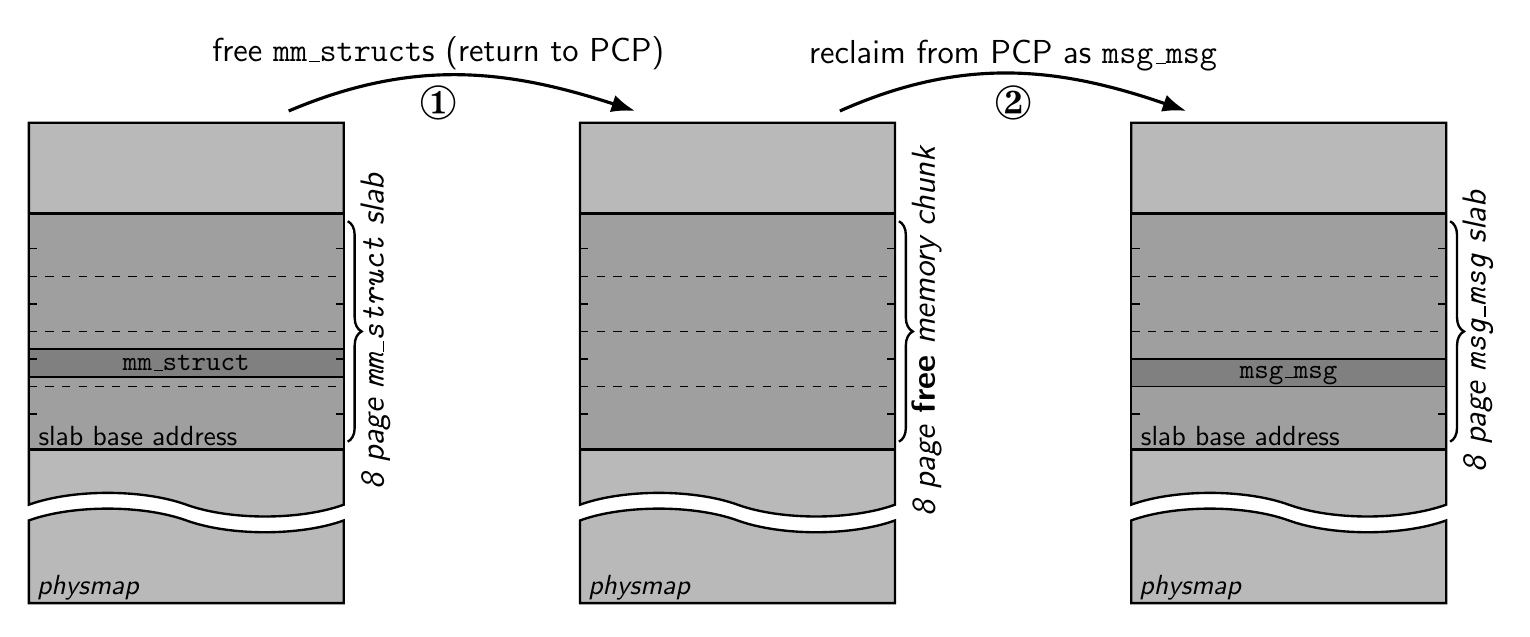
\begin{tikzpicture}

    \tikzstyle{upper}+=[
        line width = 0.3mm,
        tape,
        draw,
        tape bend top=none,
        tape bend height=3mm,
        tape bend bottom=out and in,
        minimum width=4cm,
        minimum height=5cm,
        fill=gray!12
    ]
    \tikzstyle{lower}+=[
        line width = 0.3mm,
        tape,
        draw,
        tape bend top=none,
        tape bend height=3mm,
        tape bend bottom=out and in,
        minimum width=4cm,
        minimum height=1.2cm,
        fill=gray!12,
        rotate=180
    ]
    \tikzstyle{dpmrange}+=[
        draw,
        line width = 0.3mm,
        minimum width=4cm,
        minimum height=3.5cm,
        fill=gray!30
    ]
    \tikzstyle{physmap}+=[
        draw,
        line width = 0.3mm,
        minimum width=4cm,
        minimum height=1cm,
        fill=gray!55
    ]
    \tikzstyle{objbool}+=[
        draw,
        line width = 0.3mm,
        minimum width=4cm,
        minimum height=3cm,
        fill=gray!75
    ]
    \tikzstyle{obj}+=[
        draw,
        line width = 0.22mm,
        minimum width=4cm,
        minimum height=0.35cm,
        fill=gray
    ]
    \tikzstyle{arrow}+=[
        -{Latex[length=3mm]},
        line width = 0.4mm
    ]
    \tikzstyle{iline}+=[
        dashed,
        rounded corners=0.7mm,
        line width = 0.3mm
    ]
    \tikzstyle{pageline}+=[
        iline,
        line width = 0.18mm
    ]

    % ----------------------------------------------------------------------------
    % ----------------------------------------------------------------------------
    % ----------------------------------------------------------------------------
    \coordinate(first) at (0, 0);
    \coordinate(second) at (7, 0);
    \coordinate(third) at (14, 0);

    % ----------------------------------------------------------------------------
    \draw[arrow] ([shift=(first)]1.3,2) to [out=23, in=162] ([shift=(second)]-1.3,2);
    \draw[arrow] ([shift=(second)]1.3,2) to [out=24, in=161] ([shift=(third)]-1.3,2);

    % ----------------------------------------------------------------------------
    \node[font=\large,align=center] at ([shift=(first)]3.2,2.73) {free \texttt{mm\_struct}s (return to PCP)};
    \node[font=\large,align=center] at ([shift=(second)]3.5,2.7) {reclaim from PCP as \texttt{msg\_msg}};
    \node[font=\LARGE,align=center] at ([shift=(first)]3.2,2.1) {\ding{172}};
    \node[font=\LARGE,align=center] at ([shift=(second)]3.5,2.1) {\ding{173}};

    % ----------------------------------------------------------------------------
    % ----------------------------------------------------------------------------
    % ----------------------------------------------------------------------------
    \coordinate(dpmup) at ([shift=(first)]0,-0.5);
    \coordinate(dpmdown) at ([shift=(first)]0,-3.8);
    \coordinate(objbool) at ([shift=(first)]0, -0.8);
    \coordinate(obj) at ([shift=(first)]0, -1.2);
    \draw[decorate,decoration={brace,amplitude=5pt},line width=0.3mm] ([shift=(objbool)]2.05,1.4) -- ([shift=(objbool)]2.05,-1.4);

    % ----------------------------------------------------------------------------
    \node[upper,fill=gray!55] at (dpmup) {};
    \node[lower,fill=gray!55] at (dpmdown) {};
    \node[objbool] at (objbool) {};
    \node[obj] at (obj) {};

    % ----------------------------------------------------------------------------
    \node[font=\itshape\large,rotate=90] at ([shift=(objbool)]2.4,0) {8 page \texttt{mm\_struct} slab};
    \node[font=\itshape] at ([shift=(dpmup)]-1.25,-3.55) {physmap};
    \node[] at ([shift=(obj)]0,0) {\texttt{mm\_struct}};

    % ----------------------------------------------------------------------------
    \draw[pageline] ([shift=(objbool)]-2,0) to ([shift=(objbool)]2,0);
    \draw[pageline] ([shift=(objbool)]-2,0.7) to ([shift=(objbool)]2,0.7);
    \draw[pageline] ([shift=(objbool)]-2,-0.7) to ([shift=(objbool)]2,-0.7);
    \draw[pageline] ([shift=(objbool)]-2,1.05) to ([shift=(objbool)]-1.8,1.05);
    \draw[pageline] ([shift=(objbool)]2,1.05) to ([shift=(objbool)]1.8,1.05);
    \draw[pageline] ([shift=(objbool)]-2,-1.05) to ([shift=(objbool)]-1.8,-1.05);
    \draw[pageline] ([shift=(objbool)]2,-1.05) to ([shift=(objbool)]1.8,-1.05);
    \draw[pageline] ([shift=(objbool)]-2,0.35) to ([shift=(objbool)]-1.8,0.35);
    \draw[pageline] ([shift=(objbool)]2,0.35) to ([shift=(objbool)]1.8,0.35);
    \draw[pageline] ([shift=(objbool)]-2,-0.35) to ([shift=(objbool)]-1.8,-0.35);
    \draw[pageline] ([shift=(objbool)]2,-0.35) to ([shift=(objbool)]1.8,-0.35);

    % ----------------------------------------------------------------------------
    \node[anchor=west] at ([shift=(objbool)]-2,-1.32) {slab base address};

    % ----------------------------------------------------------------------------
    % ----------------------------------------------------------------------------
    % ----------------------------------------------------------------------------
    \coordinate(dpmup) at ([shift=(second)]0,-0.5);
    \coordinate(dpmdown) at ([shift=(second)]0,-3.8);
    \coordinate(objbool) at ([shift=(second)]0, -0.8);
    \coordinate(obj) at ([shift=(second)]0, -1.2);
    \draw[decorate,decoration={brace,amplitude=5pt},line width=0.3mm] ([shift=(objbool)]2.05,1.4) -- ([shift=(objbool)]2.05,-1.4);

    % ----------------------------------------------------------------------------
    \node[upper,fill=gray!55] at (dpmup) {};
    \node[lower,fill=gray!55] at (dpmdown) {};
    \node[objbool] at (objbool) {};

    % ----------------------------------------------------------------------------
    \node[font=\itshape\large,rotate=90] at ([shift=(objbool)]2.4,0) {8 page \textbf{free} memory chunk};
    \node[font=\itshape] at ([shift=(dpmup)]-1.25,-3.55) {physmap};

    % ----------------------------------------------------------------------------
    \draw[pageline] ([shift=(objbool)]-2,0) to ([shift=(objbool)]2,0);
    \draw[pageline] ([shift=(objbool)]-2,0.7) to ([shift=(objbool)]2,0.7);
    \draw[pageline] ([shift=(objbool)]-2,-0.7) to ([shift=(objbool)]2,-0.7);
    \draw[pageline] ([shift=(objbool)]-2,1.05) to ([shift=(objbool)]-1.8,1.05);
    \draw[pageline] ([shift=(objbool)]2,1.05) to ([shift=(objbool)]1.8,1.05);
    \draw[pageline] ([shift=(objbool)]-2,-1.05) to ([shift=(objbool)]-1.8,-1.05);
    \draw[pageline] ([shift=(objbool)]2,-1.05) to ([shift=(objbool)]1.8,-1.05);
    \draw[pageline] ([shift=(objbool)]-2,0.35) to ([shift=(objbool)]-1.8,0.35);
    \draw[pageline] ([shift=(objbool)]2,0.35) to ([shift=(objbool)]1.8,0.35);
    \draw[pageline] ([shift=(objbool)]-2,-0.35) to ([shift=(objbool)]-1.8,-0.35);
    \draw[pageline] ([shift=(objbool)]2,-0.35) to ([shift=(objbool)]1.8,-0.35);


    % ----------------------------------------------------------------------------
    % ----------------------------------------------------------------------------
    % ----------------------------------------------------------------------------
    \coordinate(dpmup) at ([shift=(third)]0,-0.5);
    \coordinate(dpmdown) at ([shift=(third)]0,-3.8);
    \coordinate(objbool) at ([shift=(third)]0, -0.8);
    \coordinate(obj) at ([shift=(third)]0, -1.325);
    \draw[decorate,decoration={brace,amplitude=5pt},line width=0.3mm] ([shift=(objbool)]2.05,1.4) -- ([shift=(objbool)]2.05,-1.4);

    % ----------------------------------------------------------------------------
    \node[upper,fill=gray!55] at (dpmup) {};
    \node[lower,fill=gray!55] at (dpmdown) {};
    \node[objbool] at (objbool) {};

    % ----------------------------------------------------------------------------
    \node[font=\itshape\large,rotate=90] at ([shift=(objbool)]2.4,0) {8 page \texttt{msg\_msg} slab};
    \node[font=\itshape] at ([shift=(dpmup)]-1.25,-3.55) {physmap};

    % ----------------------------------------------------------------------------
    \node[obj] at (obj) {};
    \node[] at ([shift=(obj)]0,-0.03) {\texttt{msg\_msg}};

    % ----------------------------------------------------------------------------
    \draw[pageline] ([shift=(objbool)]-2,0) to ([shift=(objbool)]2,0);
    \draw[pageline] ([shift=(objbool)]-2,0.7) to ([shift=(objbool)]2,0.7);
    \draw[pageline] ([shift=(objbool)]-2,-0.7) to ([shift=(objbool)]2,-0.7);
    \draw[pageline] ([shift=(objbool)]-2,1.05) to ([shift=(objbool)]-1.8,1.05);
    \draw[pageline] ([shift=(objbool)]2,1.05) to ([shift=(objbool)]1.8,1.05);
    \draw[pageline] ([shift=(objbool)]-2,-1.05) to ([shift=(objbool)]-1.8,-1.05);
    \draw[pageline] ([shift=(objbool)]2,-1.05) to ([shift=(objbool)]1.8,-1.05);
    \draw[pageline] ([shift=(objbool)]-2,0.35) to ([shift=(objbool)]-1.8,0.35);
    \draw[pageline] ([shift=(objbool)]2,0.35) to ([shift=(objbool)]1.8,0.35);
    \draw[pageline] ([shift=(objbool)]-2,-0.35) to ([shift=(objbool)]-1.8,-0.35);
    \draw[pageline] ([shift=(objbool)]2,-0.35) to ([shift=(objbool)]1.8,-0.35);

    % ----------------------------------------------------------------------------
    \node[anchor=west] at ([shift=(objbool)]-2,-1.32) {slab base address};

    % ----------------------------------------------------------------------------
    \draw[pageline] ([shift=(objbool)]-2,-0.35) to ([shift=(objbool)]-1.8,-0.35);
    \draw[pageline] ([shift=(objbool)]2,-0.35) to ([shift=(objbool)]1.8,-0.35);

\end{tikzpicture}
\end{document}
